Programmable Gain Arrays (PGA) are an electronic scheme to modify on the fly the gain of a system. PGA allow an amplifier to choose from multiple values of gain resistor $R_f$.  This can be achieved with simple relays or multiplexers that can switch when toggled between different resistors \cite{Chabowski2015,horowitz1989art}. The gains are generally controllable by the MCU (see \autoref{sec:MCU}) and the PGA is generally placed in the feeback loop of an amplifier. An exemple of a PGA is provided in \autoref{fig:PGA}.
\begin{figure}[h]
    \centering
    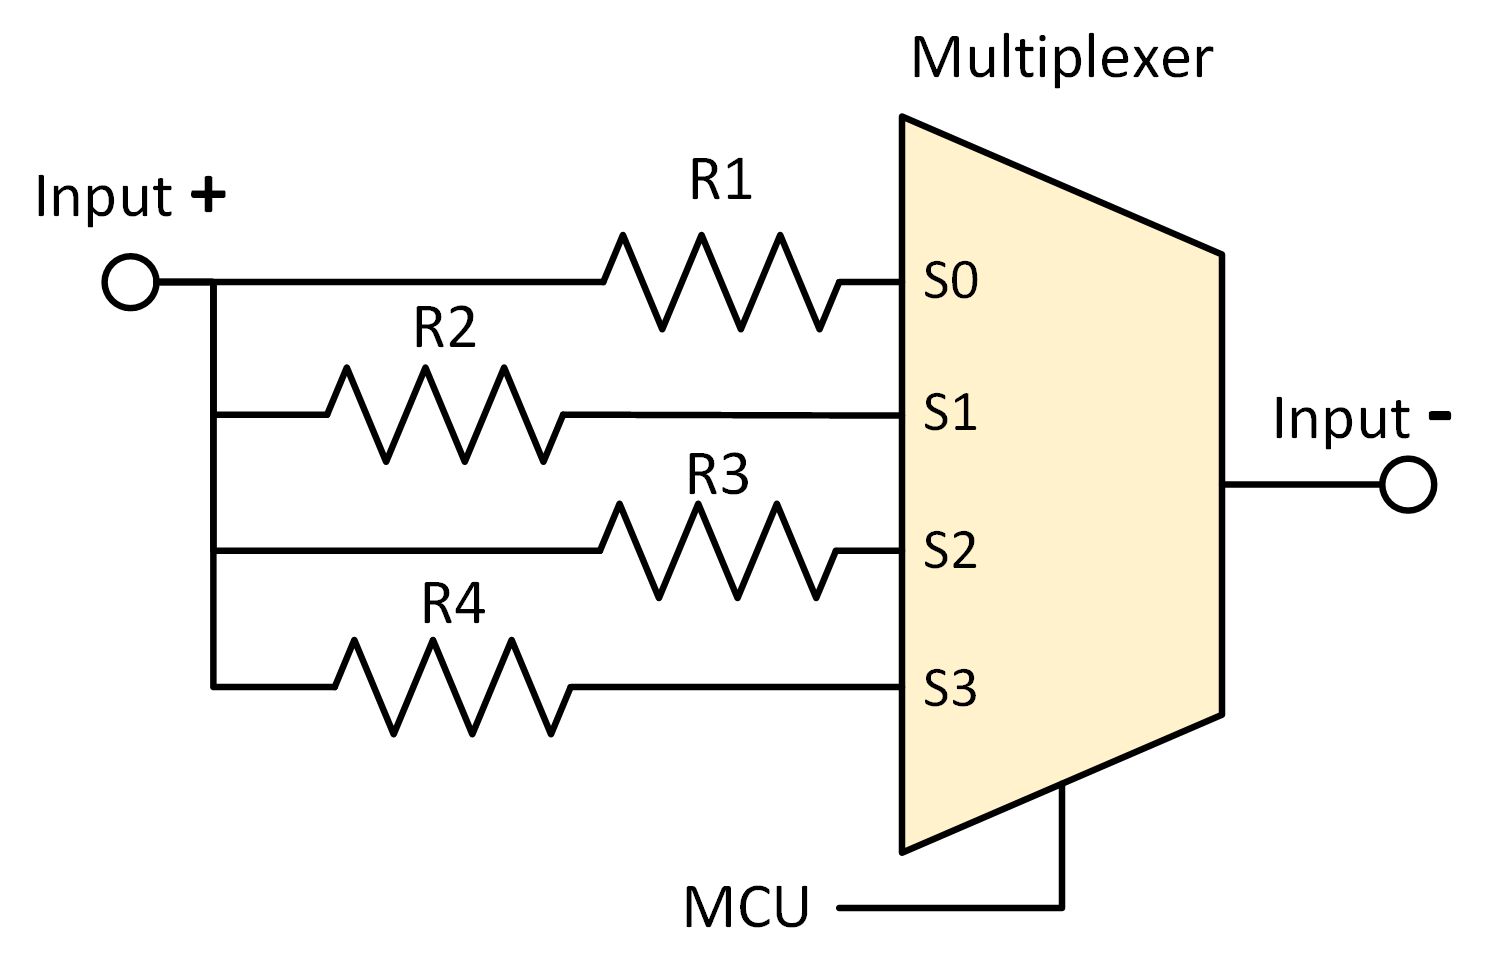
\includegraphics[width=0.7\textwidth]{PGA}
    \caption{Implementation of a PGA using switchable resistors controlled by a multiplexer.}
    \label{fig:PGA}
\end{figure}